\end{multicols}
\begin{multicols}{2}[\section{Development process}]
\label{sec:development-process}

An important subfield of software engineering is the use of known methods and principles. The development process implies the used methods and principles. Thus this section will cover the chosen development process, its ideal procedure and how the development process actual took place including a timeline of events.

\end{multicols}
\begin{multicols}{2}[\subsection{Intended development process}]
\label{sec:intended-development-process}

As mentioned above \emph{MyCourses} is the first software project for everyone in the team. The selection of a development process was heavily based on the software engineering course we heard in the summer 2010. A major part of the project was realized in the period of lectures. This and the long distances between our homes is why we decided against an agile development process, as we did not have the opportunity to communicate and meet on a daily basis.

For the intended development process we chose the spiral model \cite{spiral}. An iterative model used incrementally seemed to be promising. Dividing our project into iterations would give us a frame of orientation for the project management. The incremental working method was fitting as we were sure there will be no functioning version of the program after the first iteration. Overall the spiral model focuses on solving those problems which reduce the projects risks at best. This fact reflected our expected work habits to adressing those problems which are blocking the project accomplishment the most.

We rather chose the spiral model as the basis for our own process and assumed that adaption would become necessary. We did not, however, have a clear concept of what might require adaption and how said adaption might be realized. Further we discussed essentials which should support and promote our work-flow. Key components of our process were therefore:

\begin{itemize}
\item \ads{regular meetings} for coordination
\item communication via \ads{e-mail}
\item evaluation of every iteration
\item \ads{ticket system} for defining and monitoring tasks
\item \ads{wiki} for collaborative document creation
\end{itemize}

\end{multicols}

\pagebreak

\begin{figure}[t]
	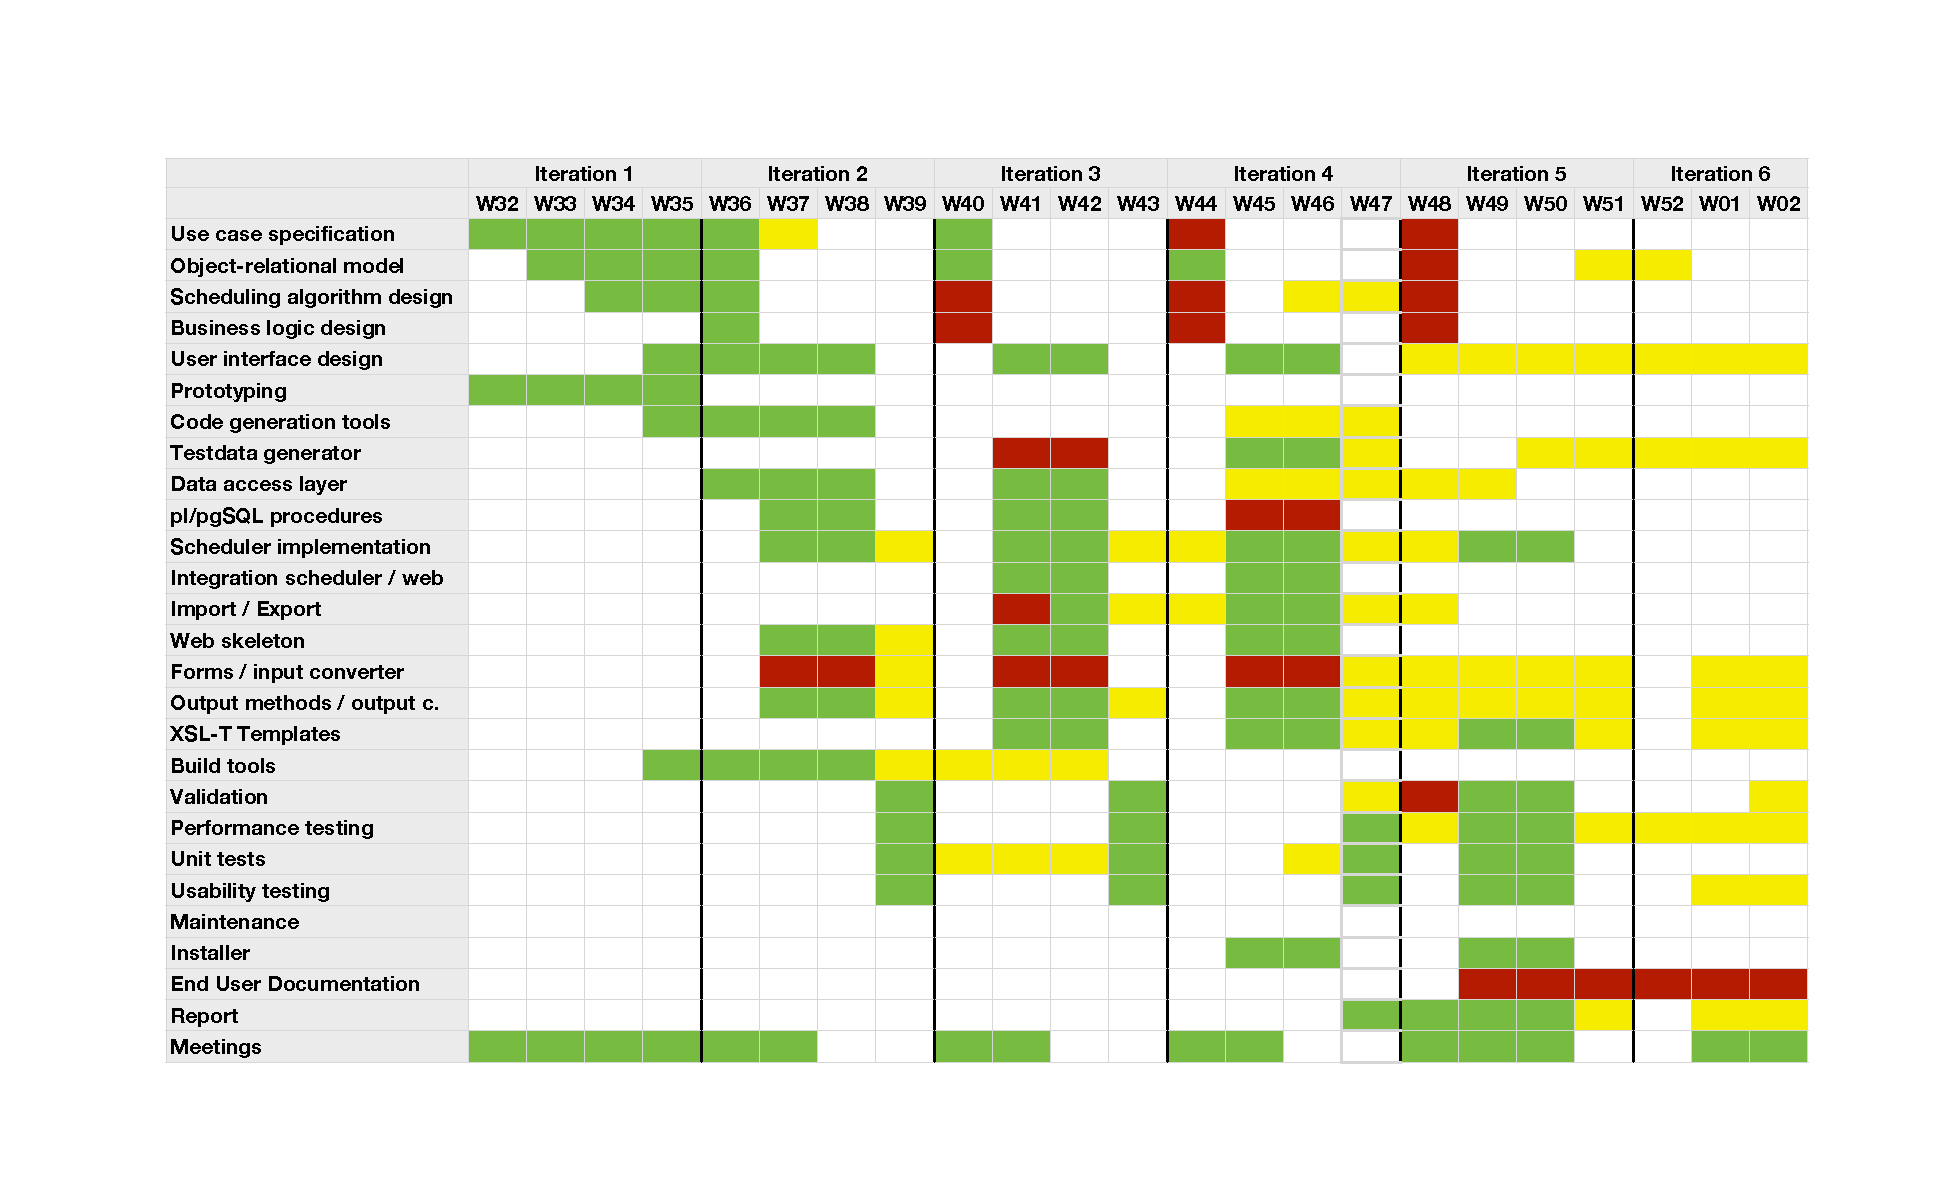
\includegraphics[width=\columnwidth]{images/gantt.pdf}
	{\color{YellowGreen} green} cells: components which we workend on as planned \\ {\color{Goldenrod} yellow} cells: components we worked on off our plan \\ {\color{BrickRed} red} cells: components we did not work on although planned
	\caption{Our project plan, originally conception and actual process}
	\label{fig:gantt-chart}
\end{figure}

\begin{multicols}{2}[\subsection{Actual development process}]
\label{sec:actual-development-process}

How the actual development process took place can be best understand when reading the timeline in section 2.3. In retrospect to the spiral model certain variations emerged. 

The beginning of every iteration is characterized by detailed requirement definitions. An intense requirement elicitation based on the \emph{MyCourses} specification was done in the first iteration with the result of a set of written use cases. In subsequent iterations, however, the requirement refinement was not done in the beginning of each iteration, but distributed over the iterations whenever problems with the current design emerged.

Even though we implemented a minimalistic prototype of \emph{MyCourses} in iteration 1, there was no continuous prototype development for comparation and evaluation as proposed by the spiral model. We focused on incremental development of the final product in every iteration.

In contrast other procedures in the development process went according to the spiral model. We put a lot of effort into the evaluation of different architectures and their resulting design. Further we tried to reduce the possible project risks by prioritizing the next main goals for the iteration.

In matters of organizing ourselves and use of methods we had a steep learning curve. In August and September we selected superordinated goals, but in the middle of each iteration we often lost focus of important tasks. The biggest improvement of the development process was therefore the introduction of weekly task assignments for every team member starting in October. Based on that, the tasks and their results were evaluated in every week, which lead to a purposeful work and swift discussion of emerging problems.



\end{multicols}
\begin{multicols}{2}[\subsection{Timeline}]
\label{sec:Timeline}
A short overview of the course our project took will be given in the next paragraphs. The goals for a phase were defined after evaluation of the previous phase had been completed. Before our project really started we got to know each other and decided which professor should be our contact person at university.

\begin{description}
\item[The First iteration] started on June 20, comprising an initial requirement elicitation, design of our software, prototyping of the scheduler and choosing technologies. During most of this time the academic term was still running and only a fraction of our time was devoted to the project. This iteration ended on September 9 and was evaluated the day before. Much of the time spent in this iteration was still focused on gaining orientation. Still it was necessary for us to take this time and find a suitable approach to the work ahead.

\item[The Second iteration] started on September 10 and was devoted to producing the scheduling algorithm, the web interface and our ORM as well as the servlet code. Work cycles were short and meetings were held every few days, including a weekend  devoted to coding. From this point on our iterations were reduced to about one month each, the focus being shifted on implementing and testing. Requirements and design were refactored whenever we felt the need to -- due to new insights or problems. This iteration ended on October 4 and was evaluated the same day.

\item[The Third iteration] accordingly started on October 5, but most work was halted until October 16 due to exams and all-day courses at university. Beginning with October 26 weekly two-hour meetings were held at our university during which everyone reported achievements and problems of the previous week. At the end of each session goals for the following week were set. These weekly meetings have proven to be a good way of coordinating work as well as motivating each other, so they were maintained for the remainder of the project. The main goal and achievement of this iteration was the integration of the scheduler with the web-interface and the connection to the database. Due to this employment of parts of our software many issues were found and fixed. Accordingly we shifted our focus further towards unit-testing and started using a tool to measure code coverage, that is how much of our code is actually being executed  as part of a unit-test. At the same time more  functionality was added to the web-interface. This iteration ended on November 1 and was evaluated the day before.

\item[The Fourth iteration] started on November 2, with the primary focus lying on the improvement of our web interface, adding functionality and a unified design. Several improvements to the scheduler algorithm were made, most notably the introduction of a greedy algorithm. Work on the summary report was also started during this iteration and the first version -- which was the basis for all further versions -- was written. The iteration ended on December 5.

\item[The Fifth iteration] started on December 6 and was mainly devoted to minor improvements to the scheduler and writing the beta-version of our summary report. One improvement to our database-access-layer which made query-caching available drastically improved scheduling performance by a factor of 8. The iteration ended on December 30.


\item[The Sixth iteration] was not part of our original project plan. The project was late and so we had to add three additional weeks for last feature implementations amd quality assurance.

\end{description}
